\documentclass[a4paper]{article}

% --- Packages ---

\usepackage{a4wide}
\usepackage[utf8]{inputenc}
\usepackage{amsmath}
\usepackage{mathtools}
\usepackage{amssymb}
\usepackage[english]{babel}
\usepackage{mdframed}
\usepackage{systeme,}
\usepackage{lipsum}
\usepackage{relsize}
\usepackage{caption}
\usepackage{tikz}
\usepackage{tikz-3dplot}
\usetikzlibrary{shapes.geometric}
\usepackage{pgfplots}
\usepackage{pgfplotstable}
\pgfplotsset{compat=newest}%1.7}
\usepackage{harpoon}%
\usepackage{graphicx}
\usepackage{wrapfig}
\usepackage{subcaption}
\usepackage{authblk}
\usepackage{float}
\usepackage{listings}
\usepackage{xcolor}
\usepackage{chngcntr}
\usepackage{amsthm}
\usepackage{comment}
\usepackage{commath}
\usepackage{hyperref}%Might remove, adds link to each reference
\usepackage{url}
\usepackage{calligra}
\usepackage{pgf}
\usepackage{isotope}

% --- Bibtex ---

\usepackage{csquotes}
\usepackage[
    %backend=biber,
    backend = biber,
    style=phys,
    sorting=ynt,
]{biblatex}

\addbibresource{ref.bib}


% --- Commands --- 

\newcommand{\w}{\omega}
\newcommand{\trace}{\text{Tr}}
\newcommand{\grad}{\mathbf{\nabla}}
%\newcommand{\crr}{\mathfrak{r}}
\newcommand{\laplace}{\nabla^2}
\newcommand{\newparagraph}{\vspace{.5cm}\noindent}

% --- Math character commands ---

\newcommand{\curl}[1]{\mathbf{\nabla}\times \mathbf{#1}}
\newcommand{\dive}[1]{\mathbf{\nabla}\cdot \mathbf{#1}}
\newcommand{\res}[2]{\text{Res}(#1,#2)}
\newcommand{\fpartial}[2]{\frac{\partial #1}{\partial #2}}
\newcommand{\rot}[3]{\begin{vmatrix}\hat{x}&\hat{y}&\hat{z}\\\partial_x&\partial_y&\partial_z\\#1&#2&#3 \end{vmatrix}}
\newcommand{\average}[1]{\langle #1 \rangle}
\newcommand{\ket}[1]{|#1\rangle}
\newcommand{\bra}[1]{\langle #1|}


%  --- Special character commands ---

\DeclareMathAlphabet{\mathcalligra}{T1}{calligra}{m}{n}
\DeclareFontShape{T1}{calligra}{m}{n}{<->s*[2.2]callig15}{}
\newcommand{\crr}{\mathcalligra{r}\,}
\newcommand{\boldscriptr}{\pmb{\mathcalligra{r}}\,}



\title{Handin 1}
\author{Author : Andreas Evensen}
\date{Date: \today}

% --- Code ---

\definecolor{codegreen}{rgb}{0,0.6,0}
\definecolor{codegray}{rgb}{0.5,0.5,0.5}
\definecolor{codepurple}{rgb}{0.58,0,0.82}
\definecolor{backcolour}{rgb}{0.95,0.95,0.92}


\lstdefinestyle{mystyle}{
    backgroundcolor=\color{backcolour},   
    commentstyle=\color{codegreen},
    keywordstyle=\color{magenta},
    numberstyle=\tiny\color{codegray},
    stringstyle=\color{codepurple},
    basicstyle=\ttfamily\footnotesize,
    breakatwhitespace=false,         
    breaklines=true,                 
    captionpos=b,                    
    keepspaces=true,                 
    numbers=left,                    
    numbersep=5pt,                  
    showspaces=false,                
    showstringspaces=false,
    showtabs=false,                  
    tabsize=2
}

\lstset{style=mystyle}

\begin{document}

%\maketitle
\input{frontpage.tex}
\tableofcontents
\section{Introduction}
\begin{comment}
In the early 20th-centary, people started to investigate the radioactive decay of elements.
The decay of an element is a random process, and it was found that the probability of a nucleus decaying in a given time interval is constant.
By experiments, it was found that the half-life, which is the rate of which half of the nuclei in the original sample has decayed, is a constant for a given isotope, differed very grately between different isotopes.
In this report, we will investigate one method to determine the half-life using quantum mechanics.
\end{comment}
In the early 20th-centary, people started to investigate the radioactive decay of elements.
The decay of an element is a random process, and there exists more than one type of decay, such as: alpha-, beta-, and gamma-decay.
The alpha decay is a process when the nuclei emit an alpha particle, which is a helium nucleus.
Scientists found a model, which describes the half-life of the nuclei, which is dependent on the kinetic energy of the outgoing alpha particle using quantum mechanics.
%In this report, one will investigate this model, and compare the results with tabulated data and see if the model is consistent with the theory.
In this report, one will investigate the model, and compare the result to the theory and tabulated data to see if the model is consistent.


\newpage
\section{Theory \& Method}
%One can think of an alpha decay such as a tunneling process; an alpha particle is emitted from the nuclei.
One can think of an alpha decay as a tunneling process; an alpha particle has to traverse a potential boundary which is higher than the kinetic energy of the particle.
This region is called the classically forbidden region.
Hence, we can view the alpha decay as a quantum mechanical process, where the alpha particle has to tunnel through the potential barrier.
We can describe the process of alpha decay using the Schrödinger equation:
\begin{align}
    i\hbar \fpartial{\psi}{t} + V(r)\psi = H\psi. \label{eq: Schrödinger}
\end{align}

\begin{figure}[H]
    \centering
    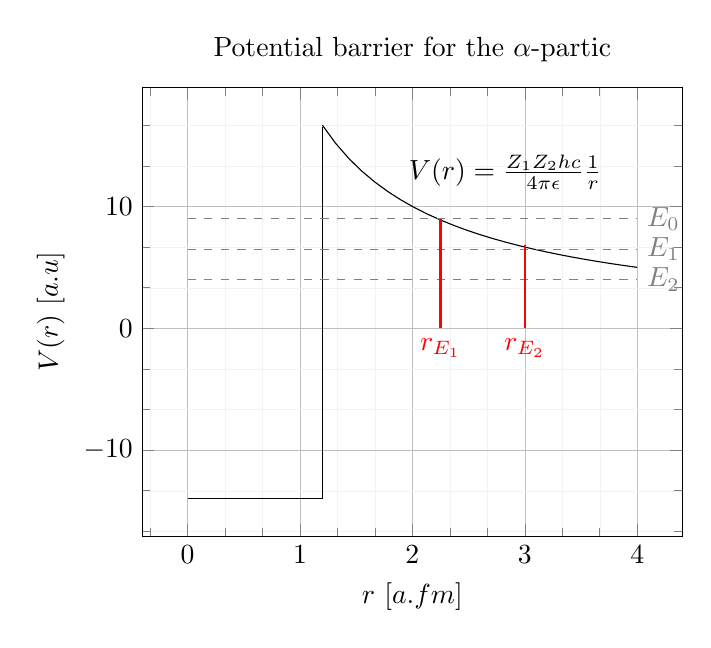
\begin{tikzpicture}
        \begin{axis}[
            xlabel = {$r ~[a.fm]$},
            ylabel = {$V(r)~[a.u]$},
            grid = both,
            grid style={line width=.1pt, draw=gray!10},
            major grid style={line width=.2pt,draw=gray!50},
            minor tick num=2,
            title = {Potential barrier for the $\alpha$-partic}
            ]
            \plot[domain = 0:1.2] {-14};   
            \plot[domain = 1.2:4] {20.0 / x} node[above right, pos = 0.5] {$V(r) = \frac{Z_1Z_2 hc}{4\pi \epsilon}\frac{1}{r}$};
            \draw (1.2, -14) -- (1.2, 16.5);
            \draw[dashed, gray] (0, 9) -- (4, 9) node[right] {$E_0$};
            \draw[dashed, gray] (0, 6.5) -- (4, 6.5) node[right] {$E_1$};
            \draw[dashed, gray] (0, 4) -- (4, 4) node[right] {$E_2$};
            \draw[red, thick] (3, 0) -- (3, 6.85) node[below, pos = 0] {$r_{E_2}$};
            \draw[red, thick] (2.25, 0) -- (2.25, 9) node[below, pos = 0] {$r_{E_1}$};
        \end{axis}
    \end{tikzpicture}
    %\includegraphics[width=0.5\textwidth]{code/potential_energy.png}
    \caption{Potential barrier for alpha decay.}
    \label{fig: alpha_decay}
\end{figure}\noindent
In the above figure, \ref{fig: alpha_decay}, we see the potential barrier for alpha decay.
The potential barrier, $V(r)$ (the Columb repulsion) is discretized into $n$ regions, where we assume that the potential is constant across those regions.
This leads to the following equations:
\begin{align}
    \psi_i(r) &= A_i e^{k_ir} + B_i e^{-k_ir}, \quad r \in (r_{i}, r_{i + 1}], \quad i = 1,2,...,n - 1, \label{eq: wavefunction}\\
    \psi_n(r) &= A_n e^{k_n r}, \quad r \in (r_{n-1}, \infty), \nonumber%\label{eq: wavefunction2}
\end{align}The last wave function, $\psi_n$, is just the outgoing wave, since we assume no barrier for $r > r_{n-1}$. In the definition above, we defined the wave-number, $k_i$ to be the following:
\begin{align}
    k_i = \frac{\sqrt{2mc^2(E-V_i)}}{\hbar c}, \quad i = 1,2,...,n, \label{eq: wave_number}
\end{align}where $V_i$ is the potential in the $i$-th region.
%For the wave-function to be continuous and differentiable, we require that the wave functions $\psi_i = \psi_{i + 1}$ at the boundaries interfacing the two wave-functions.
For the wave-function to be well-defined for this problem, the wave-functions at the interfaces must be equal, and also there derivatives, $\psi_i = \psi_{i+1}$ at $r_i$ and $\psi_i' = \psi_{i+1}'$ at $r_i$.
%Moreover, the derivative of the wave function must also be continuous at the boundaries, hence we get the following matrix equation:
Solving the above equations, we get the following matrix equation:
\begin{align}
    \begin{pmatrix}
        1 & 0 & 0 & 0 & \hdots & 0 & 0 & 0\\
        e^{ik_1r_1} & e^{-ik_1r_1} & -e^{ik_2r_1} & -e^{-ik_2r_1}& \hdots & 0 & 0 & 0\\
        ik_1e^{ik_1r_1} & -ik_1e^{-ik_1r_1} & -ik_2e^{ik_2r_1} & ik_2e^{-ik_2r_1} & \hdots & 0 & 0 & 0\\
        \vdots&\ddots&\ddots&\ddots&\ddots&\ddots&\ddots&\vdots
        %0 & 0 & 0 & 0 & 0 & e^{ik_{n-1}r_{n-1}} & e^{-ik_{n-1}r_{n-1}} & e^{ik_nr_{n-1}}\\
        %0 & 0 & 0 & 0 & 0 & ik_{n-1}e^{ik_{n-1}r_{n-1}} & -ik_{n-1}e^{-ik_{n-1}r_{n-1}} & ik_ne^{ik_nr_{n-1}}
    \end{pmatrix}\cdot\mathbf{x} = \begin{pmatrix}
        1\\
        0\\
        0\\
        \vdots
        %0\\
        %0
    \end{pmatrix},\label{eq: matrix eq}
\end{align}where $\mathbf{x}$ is a vector containing the coefficients $A_i$ and $B_i$. This matrix equation can be solved using various numerical techniques, such as:
LU factorization, incomplete Chavosky factorization, or Gaussian elimination.

\newparagraph
The unity equation is thus composed by the reflection and transmission probabilities, and in our system that is reflected as:
\begin{align}
    1 = \abs{\frac{B_1}{A_1}}^2 + \abs{\frac{A_n}{A_1}}^2\frac{k_n}{k_1},\label{eq: transmission_probability}
\end{align}where $A$, $B$ are the elements in our unknown in equation \eqref{eq: matrix eq}. The $k$'s are then the wave-functions wave-number.
Using this, one derives the half life of the system as the oscillation frequency of the wave-function, which takes into account the masses of the system, and the kinetic energy of the outgoing $\alpha$-particle:
\begin{align}
    t_{1/2} = \ln(2)\frac{T\cdot v}{2R},\label{eq: half-life}
\end{align}where $T$ is the transmission probability, $v$ is the effective velocity of the system, and $R$ is the radii of the nuclei\cite{krane1991introductory}. Below is a figure to visualize our discretization of the system:

\begin{figure}[H]
    \centering
    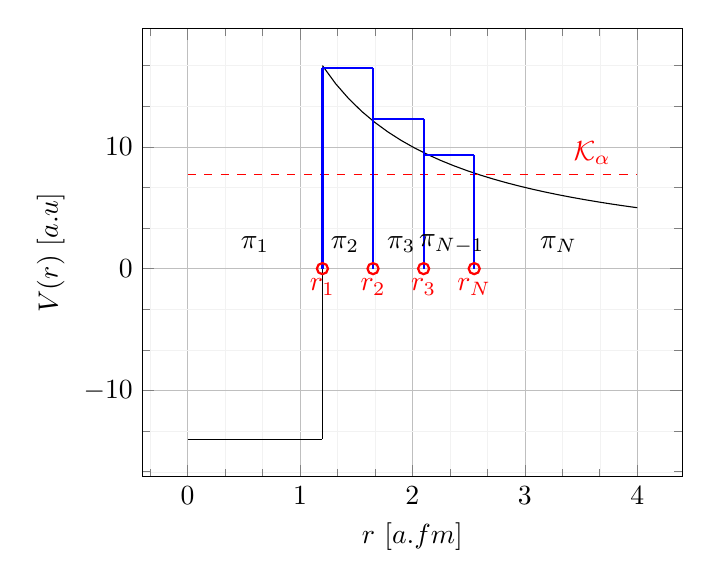
\begin{tikzpicture}
        \begin{axis}[
            xlabel = {$r ~[a.fm]$},
            ylabel = {$V(r)~[a.u]$},
            grid = both,
            grid style={line width=.1pt, draw=gray!10},
            major grid style={line width=.2pt,draw=gray!50},
            minor tick num=2,
            ]
            \plot[domain = 0:1.2] {-14};   
            \plot[domain = 1.2:4] {20.0 / x};% node[above right, pos = 0.5] {$V(r) = \frac{Z_1Z_2 hc}{4\pi \epsilon}\frac{1}{r}$};
            \draw (1.2, -14) -- (1.2, 16.5);
            \draw[dashed, red] (0, 7.75) -- (4, 7.75) node[above, pos = 0.9] {$\mathcal{K}_\alpha$};

            \draw[blue, thick] (1.2,0) -- (1.2, 16.5);
            \draw[blue, thick] (1.2, 16.5) -- (1.2 + .45, 16.5);
            \draw[blue, thick] (1.2 + 0.45,0) -- (1.2 + 0.45, 16.5);

            \draw[blue, thick] (1.2 + 0.45 * 2,0) -- (1.2 + 0.45 * 2, 12.3);
            \draw[blue, thick] (1.2 + 0.45, 12.3) -- (1.2 + 0.45 * 2, 12.3);

            \draw[blue, thick] (1.2 + 0.45 * 2, 9.3) -- (1.2 + 0.45 * 3, 9.3);
            \draw[blue, thick] (1.2 + 0.45 * 3,0) -- (1.2 + 0.45 * 3, 9.3);
        

            \draw[red, thick]  (3 - 0.45, 0) circle (2pt) node[below] {$r_{N}$};
            \draw[red, thick]  (3 - 0.45 * 2, 0) circle (2pt) node[below] {$r_{3}$};
            \draw[red, thick]  (3 - 0.45 * 3, 0) circle (2pt) node[below] {$r_{2}$};
            \draw[red, thick]  (3 - 0.45 * 4, 0) circle (2pt) node[below] {$r_{1}$};

            \node at (0.6, 2) {$\pi_1$};
            \node at (1.4, 2) {$\pi_2$};
            \node at (1.9, 2) {$\pi_3$};
            \node at (2.35, 2) {$\pi_{N- 1}$};
            \node at (3.3, 2) {$\pi_{N}$};

        \end{axis}
    \end{tikzpicture}
    %\includegraphics[width=0.5\textwidth]{code/potential_energy.png}
    \caption{Visualization of the discretization process.}
    \label{fig: concept}
\end{figure}\noindent
The above figure, \ref{fig: concept}, shows the discretization of the potential barrier, where the potential is constant in each region.
Here, the radii $r_1$ is the size of the daughter nuclei, and $r_N$ is the length of which the potential barrier is greater than the kinetic energy.
The $N$ regions all then have constant potential, and in region $\pi_1$, and $\pi_N$, the wave function is defined to oscillate.


\begin{comment}
\newparagraph
The kinematics of the system leads to the following expression for the kinetic energy of the outgoing $\alpha$-particle:
\begin{align*}
    \mathcal{K} &= \frac{1}{2}m_\mu v_{eff}^2,
\end{align*}where $m_\mu$ is the reduced mass of the $\alpha$-particle and the daughter nuclei, and $v_{eff}$ is the effective velocity of the system.
\end{comment}

\newpage
\section{Implementation \& Results}
The above theory was implemented in a C++ program\ref{sec: Appendix}, where the matrix equation \eqref{eq: matrix eq} was solved.
Using the coefficient $A_0$ and $A_n$, we computed the transmission probabilities for various nuclei, which in turn derived the half-life as per equation \eqref{eq: half-life} as shown in the figure below.
\begin{figure}[H]
    \centering
    \begin{tikzpicture}[]
        \begin{semilogyaxis}[
            xlabel = {$\mathcal{K}~ [MeV]$},
            ylabel = {$t_{1/2} ~[s]$},
            grid = both,
            grid style={line width=.1pt, draw=gray!10},
            major grid style={line width=.2pt,draw=gray!50},
            minor tick num=2,
            title = {Half-life as a function of $\mathcal{K}$},
            %colormap = {black}{
            %    color(0cm) = (black);
            %    color(1cm) = (black);
            %},
            nodes near coords,
            nodes near coords style={font = \tiny},
            ]
            \addplot+[scatter, only marks, scatter src = explicit symbolic]
            table [x=K,y=t, meta = name] {code/data.dat};
        \end{semilogyaxis}
    \end{tikzpicture}
    \caption{Half life as a function of $\mathcal{K}$ for various nuclei with $r_0 = 1.4$~fm \\and $100$ number of bins.}
\end{figure}\noindent
The above figure exhibits the half-life difference between different nuclei depending on the kinetic energy of the outgoing $\alpha$-particle.
With small differences in the kinetic energy, the half-life can differ by several orders of magnitude, as visualized in the above figure.
The results are not consistent with tabulated data, which is shown in the table below \ref{tab: half-life}.
However, the results are consistent with the theory, as the half-life is dependent on the kinetic energy of the outgoing $\alpha$-particle.
\begin{figure}[H]
    \begin{minipage}[b]{.45\linewidth}
      \centering
        \begin{tikzpicture}[scale = 0.7]
            \begin{semilogyaxis}[
                xlabel = {$\mathcal{K}~ [MeV]$},
                ylabel = {$t_{1/2} ~[s]$},
                grid = both,
                grid style={line width=.1pt, draw=gray!10},
                major grid style={line width=.2pt,draw=gray!50},
                minor tick num=2,
                title = {Half-life as a function of $\mathcal{K}$},
                %colormap = {black}{
                %    color(0cm) = (black);
                %    color(1cm) = (black);
                %},
                nodes near coords,
                nodes near coords style={font = \tiny},
                ]
                \addplot+[scatter, only marks, scatter src = explicit symbolic]
                table [x=K,y=t, meta = name] {code/tab.dat};
            \end{semilogyaxis}
        \end{tikzpicture}
    \caption{Half-life as a function of $\mathcal{K}$ for various nuclei for tabulated values\cite{nist}.}
    
    \end{minipage}\hfill
    \begin{minipage}[b]{.45\linewidth}
      \centering
      \begin{tabular}{|c|c|}\hline
        Nuclei& Half-life [s]\\ \hline
        %\isotope[250][98]{Cf}& $4.1\cdot10^{8}$\\\hline
        \isotope[238][92]{U} & $1.4\cdot10^{17}$\\\hline
        \isotope[232][90]{Th} & $4.4\cdot10^{17}$ \\\hline
        \isotope[226][88]{Ra} & $5.5\cdot10^{10}$ \\\hline
        \isotope[222][86]{Rn} & $3.3\cdot10^{5}$\\\hline
        \isotope[219][86]{Rn} & $3.96$\\\hline
        \isotope[214][82]{Po} & $164\cdot10^{-6}$\\\hline
    \end{tabular}
    \caption{Half-life for various isotopes from tabulated data\cite{nist}.}
    \label{tab: half-life}
    \end{minipage}
\end{figure}\newpage\noindent
\begin{comment}
\begin{table}[H]
    \centering
    \caption{Half-life of different nuclei\cite{nist}}
    \begin{tabular}{|c|c|}\hline
        Nuclei& Half-life [s]\\ \hline
        %\isotope[250][98]{Cf}& $4.1\cdot10^{8}$\\\hline
        \isotope[238][92]{U} & $1.4\cdot10^{17}$\\\hline
        \isotope[232][90]{Th} & $4.4\cdot10^{17}$ \\\hline
        \isotope[226][88]{Ra} & $5.5\cdot10^{10}$ \\\hline
        \isotope[222][86]{Rn} & $3.3\cdot10^{5}$\\\hline
        \isotope[219][86]{Rn} & $3.96$\\\hline
        \isotope[214][82]{Po} & $164\cdot10^{-6}$\\\hline
    \end{tabular}
    \label{tab: half-life}
\end{table}\noindent
\begin{figure}[H]
    \centering
    \begin{tikzpicture}[]
        \begin{semilogyaxis}[
            xlabel = {$\mathcal{K}~ [MeV]$},
            ylabel = {$t_{1/2} ~[s]$},
            grid = both,
            grid style={line width=.1pt, draw=gray!10},
            major grid style={line width=.2pt,draw=gray!50},
            minor tick num=2,
            title = {Half-life as a function of $\mathcal{K}$},
            %colormap = {black}{
            %    color(0cm) = (black);
            %    color(1cm) = (black);
            %},
            nodes near coords,
            ]
            \addplot+[scatter, only marks, scatter src = explicit symbolic]
            table [x=K,y=t, meta = name] {code/tab.dat};
        \end{semilogyaxis}
    \end{tikzpicture}
    \caption{Tabulated half life.}
\end{figure} 
\end{comment}
In the calculations, we had two free parameters, the number of bins, and the scaling of the radii, $r_0$.
Varying the radii scaling, $r_0$, and the number of bins, we found that the half-life was very sensitive to the radii scaling, as shown in the figure below.
\begin{figure}[H]
    \centering
    \begin{subfigure}{0.45\textwidth}    
        \begin{tikzpicture}[scale = 0.75]
            \begin{semilogyaxis}[
                xlabel = {Number of bins},
                ylabel = {$t_{1/2} ~[s]$},
                grid = both,
                grid style={line width=.1pt, draw=gray!10},
                major grid style={line width=.2pt,draw=gray!50},
                minor tick num=2,
                title = {Half-life of \isotope[238][92]{U} as a function of bin size},
                legend pos = south east,
            ]
            \addplot[black, only marks] table [x = binSize, y = t] {code/data_u-238_1.400000.dat};
            \addlegendentry{$r_0 = 1.4$}
            \addplot[blue, only marks] table [x = binSize, y = t] {code/data_u-238_1.300000.dat};
            \addlegendentry{$r_0 = 1.3$}
            \addplot[red, only marks, ] table [x = binSize, y = t] {code/data_u-238_1.200000.dat};
            \addlegendentry{$r_0 = 1.2$}
            \end{semilogyaxis}
        \end{tikzpicture}
        \caption{Half life of \isotope[238][92]{U} with varying bin size.}
        \label{fig: u-238}
    \end{subfigure}
    \hfill
    \begin{subfigure}{0.45\textwidth}    
        \begin{tikzpicture}[scale = 0.75]
            \begin{semilogyaxis}[
                xlabel = {Number of bins},
                ylabel = {$t_{1/2} ~[s]$},
                grid = both,
                grid style={line width=.1pt, draw=gray!10},
                major grid style={line width=.2pt,draw=gray!50},
                minor tick num=2,
                title = {Half-life of \isotope[232][90]{Th} as a function of bin size},
                legend pos = south east,
            ]
            \addplot[purple, only marks] table [x = binSize, y = t] {code/data_th-232_1.500000.dat};
            \addlegendentry{$r_0 = 1.5$}
            \addplot[black, only marks] table [x = binSize, y = t] {code/data_th-232_1.400000.dat};
            \addlegendentry{$r_0 = 1.4$}
            \addplot[blue, only marks] table [x = binSize, y = t] {code/data_th-232_1.300000.dat};
            \addlegendentry{$r_0 = 1.3$}
            \addplot[red, only marks, ] table [x = binSize, y = t] {code/data_th-232_1.200000.dat};
            \addlegendentry{$r_0 = 1.2$}
            \end{semilogyaxis}
        \end{tikzpicture}
        \caption{Half life of \isotope[232][90]{Th} with varying bin size.}
        \label{fig: th-232}
    \end{subfigure}
    \caption{Half life of \isotope[238][92]{U} and \isotope[232][90]{Th} with varying bin size.}
    \label{fig: u-238_th-232}
\end{figure}\noindent
\begin{comment}
As from the above figure, it can be seen that the half-life is very sensitive to the radii scaling $r_0$.
In both \ref{fig: u-238} -- \ref{fig: th-232} the half life increases as the number of bins increases, until it peaks and then converges.
This is due to the discretization of the potential barrier, where the potential is constant in each region, with increasing number of bins, the potential is more accurately described;
with a better description of the potential, the system is more accurately described.
\end{comment}
From the above figure, it can be seen that the half-life is very sensitive to the radii scaling $r_0$.
This is expected, as the radii scaling determines the width of classically forbidden region, and thus affects the transmission probability.
In both figures \ref{fig: u-238} and \ref{fig: th-232}, the half-life increases as the bin width decreases until it peaks and then converges.
This indicates that the bin size has to be below a certain threshold to accurately describe the potential barrier, and thus the system.

\newparagraph
The potential depth $V_0$ was also varied, and it was found that it had little impact on the half-life, as shown in the figure below.
\begin{figure}[H]
    \centering
    \begin{subfigure}{0.45\textwidth}    
        \begin{tikzpicture}[scale = 0.75]
            \begin{semilogyaxis}[
                xlabel = {$\mathcal{K}$~[MeV]},
                ylabel = {$t_{1/2} ~[s]$},
                grid = both,
                grid style={line width=.1pt, draw=gray!10},
                major grid style={line width=.2pt,draw=gray!50},
                minor tick num=2,
                title = {Half life for various nuclei with $r_0 = 1.4$~fm, $V_0 = 200$ MeV},
                legend pos = south east,
                nodes near coords,
                nodes near coords style = {font = \tiny},
            ]
            \addplot+[scatter, only marks, scatter src = explicit symbolic]
            table [x=K,y=t, meta = name] {code/data_200.000000.dat};
            \end{semilogyaxis}
        \end{tikzpicture}
        \caption{Half life of various nuclei with $V_0 = 200$ MeV.}
        \label{fig: V0 200}
    \end{subfigure}
    \hfill
    \begin{subfigure}{0.45\textwidth}    
        \begin{tikzpicture}[scale = 0.75]
            \begin{semilogyaxis}[
                xlabel = {$\mathcal{K}$~[MeV]},
                ylabel = {$t_{1/2} ~[s]$},
                grid = both,
                grid style={line width=.1pt, draw=gray!10},
                major grid style={line width=.2pt,draw=gray!50},
                minor tick num=2,
                title = {Half-life for various nuceli with $r_0 = 1.4$~fm, $V_0 = 300$ MeV},
                legend pos = south east,
                nodes near coords,
                nodes near coords style = {font = \tiny},
            ]
            \addplot+[scatter, only marks, scatter src = explicit symbolic]
            table [x=K,y=t, meta = name] {code/data_300.000000.dat};
            \end{semilogyaxis}
        \end{tikzpicture}
        \caption{Half life of various nuclei with $V_0 = 300$ MeV.}
        \label{fig: v0 300}
    \end{subfigure}
    \caption{Half life for varying potential depth.}
    \label{fig: varing potential}
\end{figure}\noindent
Hence, as the potential depth $V_0$ has little impact on the half-life, we can state that the leading parameters are the radii, the kinetic energy and the potential itself.


\section{Conclusion}
In this report, a simple model for describing the half life of nuclei which decays via alpha decay was implemented.
The results were consistent with the theory, as the half-life was dependent on the kinetic energy of the outgoing $\alpha$-particle;
however, the results were not consistent with tabulated data.
There exists multiple reasons for this, such as the discretization of the potential, the initial radii scaling and an incomplete model.
In this model, we do not take into account the spin of the nuclei, the angular momentum, or the parity of the system, which all affects the half-life.

\newparagraph
In order to further improve the model, one could take into account the factors mentioned above, such as: angular momentum and parity.
This would lead to a more accurate description of the system, and thus as a result, a more accurate model.
When solving the matrix equation, partial LU factorization was used\cite{eigenweb}, which is a very efficient method for solving the matrix equation;
however, different solver techniques were used, and the results differed significantly, which could be further investigated.
Furthermore, the model could be improved by instead of using a constant potential in each region, one could use a trapezoid method to describe the potential within the regions more accurately.

\newpage
\printbibliography


\section*{Appendix}\label{sec: Appendix}
\lstinputlisting[language = {c++}]{code/main.cpp}

\end{document}